\section{Emergency stroke pathway under study}

This project focused on use of thrombolysis and outcomes (with and without thrombolysis) at discharge from in-patient care. Figure \ref{fig:flow} shows an overview of the process steps included in the modelling. All modelling data came from the national stroke registry for England, Wales and Northern Ireland, the Sentinel Stroke National Audit Programme (SSNAP).

\begin{itemize}

    \item \textit{Stroke onset}: When known, SSNAP records the time of stroke onset.

    \item \textit{Convey to hospital}: SSNAP records the time of arrival at hospital, and records whether the arrival was by ambulance or not. For some patients there is a breakdown of ambulance response times (time of call, time of ambulance arrival on scene, time of departure from scene, time of arrival at hospital).

    \item \textit{Gather info \& determine stroke onset time}: SSNAP records whether onset time was determined, and whether it was considered to be known \textit{precisely} or was \textit{a best estimate}. Other patient information is gathered (such as recording age, sex, the NIH Stroke Scale scores, estimation of pre-stroke disability, key medications being taken by the patient). This clinical information may be taken prior to and/or after head imaging, but we restricted information for modelling treatment decisions to that information available at the time of the decision.

    \item \textit{Head scan}: Head imaging is essential to confirm stroke, and determine stroke type (ischaemic or hemorrhagic). SSNAP records whether head imaging was performed, and the time of imaging. For modelling work described here we did not request, and do not use, the mode of imaging; all modes should provide confirmation of stroke and should distinguish ischaemic and hemorrhagic stroke. 

    \item \textit{Decision to treat}: We model each stroke teams patterns of who they decide to treat with thrombolysis.

    \item \textit{Thrombolysis (IVT)}: SSNAP records whether thrombolysis was given and the time of thrombolysis.

    \item \textit{Disability at discharge}: SSNAP records modified Rankin Scale (mRS) at discharge from inpatient care. For about third of patients there is a follow-up measure at 6 months. In our modelling we use disability at discharge as (1) data is essentially complete, and (2) this is the outcome most closely tied with the effect of thrombolysis, which is our focus of study in the described project.

\end{itemize}

\begin{figure}[ht!]
    \centering
    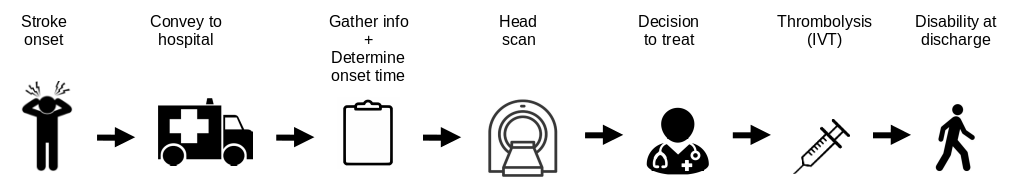
\includegraphics[width=1.0\linewidth]{images/flow}
    \caption{An overview of the process steps included in the modelling.}
    \label{fig:flow}
\end{figure}

Process flow was modelled by sampling from distributions of historic flow for each stroke team. Decision-making (choice of thrombolysis) was modelled with machine learning, learning which patients would likely be given thrombolysis at each stroke team. Outcomes were predicted using either mathematical models based on clinical trials (for the full pathway model), or clinical outcome machine learning models (for the more detailed analysis of differences in thrombolysis decision-making between teams).
